\documentclass[12pt,a4paper]{article}

\usepackage{a4wide}
\usepackage{minted}
\usepackage{csvsimple}
\usepackage{amsmath}
\usepackage{booktabs}
\usepackage{amssymb}
\usepackage{nicefrac}
\usepackage{enumitem}
\usepackage{float}
\usepackage{todonotes}
\usepackage[breaklinks,plainpages=false,pdfpagelabels]{hyperref}
\hypersetup{colorlinks,citecolor=blue,filecolor=blue,linkcolor=blue,urlcolor=blue}
\usepackage{graphicx}
\setlength\parindent{0pt} % no paragraph indents
\setlength\parskip{6pt} % paragraph vertical spacing
\usepackage{circuitikz} % for circuit diagrams
\usepackage{pgfplots}
\usepackage{tikz}
\usetikzlibrary{positioning,shapes,shadows,arrows,calc}
\DeclareMathOperator{\sinc}{sinc} %sinc
\usepackage[normalem]{ulem} %strike out text using \sout

\usepackage{fancyhdr}
\pagestyle{fancy}
\fancyhead[L]{CSSE4010: Digital Doo-Hickeys}
\fancyhead[R]{Sem 2, 2023}


%---------------------------------------------------------------%
%                                                               %
%               environment definitions                         %
%                                                               %
%---------------------------------------------------------------%
\newcounter{boldalphcounter}
\renewcommand{\theboldalphcounter}{(\alph{boldalphcounter})}
\newenvironment{boldalphlist}{\begin{list}{\textbf{\theboldalphcounter}}%
  {\usecounter{boldalphcounter}}}{\end{list}}

\newcounter{alphcounter}
\renewcommand{\thealphcounter}{(\alph{alphcounter})}
\newenvironment{alphlist}{\begin{list}{\thealphcounter}%
  {\usecounter{alphcounter}}}{\end{list}}

\newcounter{romancounter}
\renewcommand{\theromancounter}{\roman{romancounter})}
\newenvironment{romanlist}{\begin{list}{\textbf{\theromancounter}}%
  {\usecounter{romancounter}}}{\end{list}}

\newcounter{boldarabiccounter}
\renewcommand{\theboldarabiccounter}{\arabic{boldarabiccounter}}
\newenvironment{boldarabiclist}{\begin{list}{\textbf{\theboldarabiccounter.}}%
  {\usecounter{boldarabiccounter}}}{\end{list}}

 % Counter
\newcounter{questioncounter}

\begin{document}

\begin{center}
\bigskip
\section*{CSSE4010 A4}
\end{center}

David Gaul

s4671313

Lab Session: Wednesday 10-12

Submission Date: 19th-ish September

\section{Introduction}

Prac 4 required the creation of a finite state machine (FSM) that would generate a high output for two clock cycles when a consecutive sequence of "11001" was input into it. This could be approached with two different methods

\begin{itemize}
    \item Creating a singular FSM that would check that the correct sequence had been input, as well as keeping track of the number of clock cycles on the output
    \item Developing two inter-linked FSMs. One for checking for the correct sequence, the other to keep track of the number of clock cycles
\end{itemize}

I'm trying to stay positive about how interesting this report is going to be. 

But I'm boring. 

I run out of things to say after the first date. And now we're up to the fourth. 

Prepare for a report that's as bland as my soul.

\section{State and Block Diagrams}

Since it was possible to approach this design problem with two separate methods, both should be addressed with relevant state diagrams. The system containing the single FSM is described in figure \ref{fig:single_fsm}.

\begin{figure}[H]
    \centering
    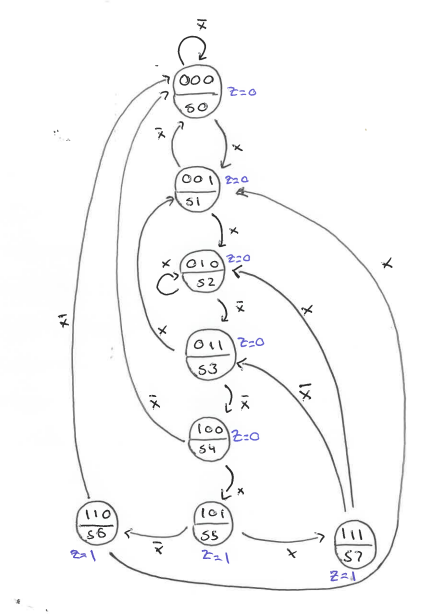
\includegraphics[scale=1]{images/single_fsm.png}
    \caption{State diagram of the system employing a singular FSM}
    \label{fig:single_fsm}
\end{figure}

A fair bit of complexity can be observed within the design of a singular FSM. Due to the heavy inter-linking of states and reliance on previous states, this model becomes difficult to scale appropriately. Although it would perform the task, its flexibility is heavily limited. For this reason, a design employing two FSMs was proposed. The state diagram for this design can be found in figure \ref{fig:double_fsm}

\begin{figure}[H]
    \centering
    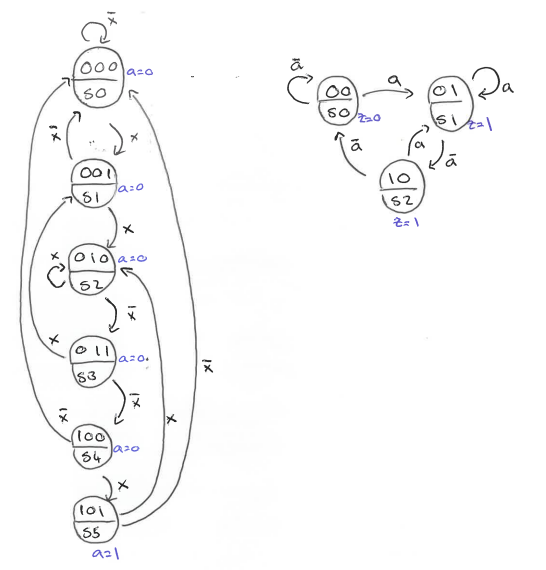
\includegraphics[scale=1]{images/double_fsm.png}
    \caption{State diagram of the system employing two FSMs}
    \label{fig:double_fsm}
\end{figure}

The second design was ultimately implemented, and will be discussed for the remainder of the report. To implement the state diagram within Xilinx, a design architecture was adopted to accommodate for a sequence detector as well as the clock counter. The block diagram for this architecture can be found within figure \ref{fig:block_diagram}

\begin{figure}[H]
    \centering
    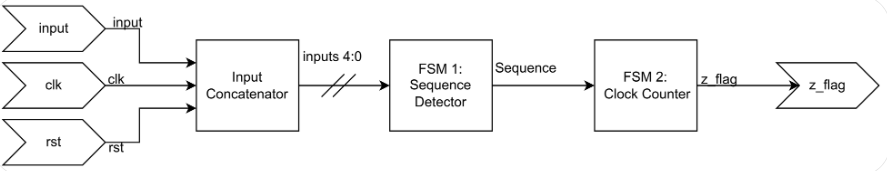
\includegraphics[scale=0.25]{images/block_diagram.png}
    \caption{Block diagram representation of the design architecture}
    \label{fig:block_diagram}
\end{figure}


\section{Simulation Results}

Several test cases had to be evaluated during simulation. The full set of tests that were run, and will be explored are as follows:

\begin{itemize}
    \item A base test case receiving 11001, with no overlap and no reset
    \item A test case receiving 11001 with no overlap, but receiving a reset
    \item A test case receiving an input of 1011001010 to test for detection in the middle of a sequence
    \item A test case receiving an overlapping input of 110011001 with no reset
    \item A test case receiving an overlapping input of 110011001 with a reset in the middle
\end{itemize}

The full range of test cases can be found in figures \ref{fig:no_overlap_no_reset}, \ref{fig:no_overlap_reset}, \ref{fig:10_sequence}, \ref{fig:overlap_no_reset} and  \ref{fig:overlap_reset}.

\begin{figure}[H]
    \centering
    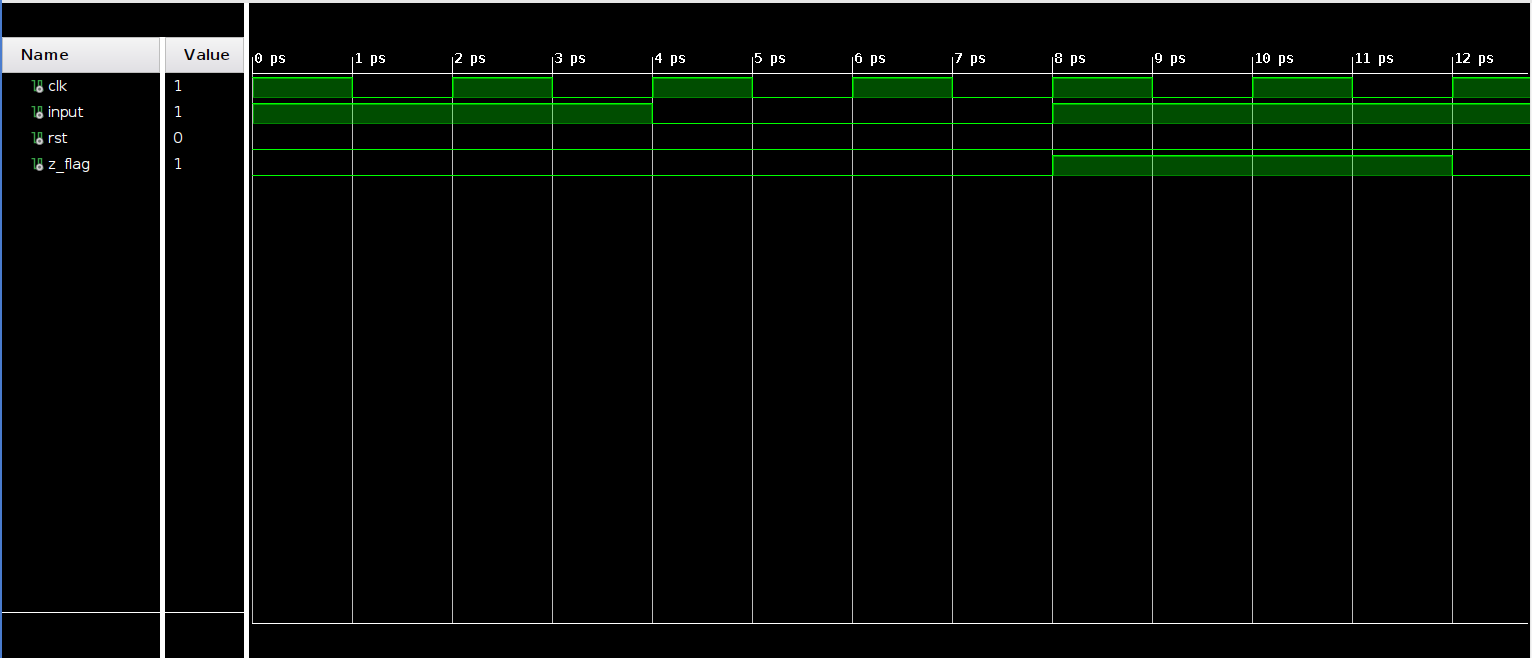
\includegraphics[scale=0.25]{images/no_overlap_no_reset.png}
    \caption{Simulation results of a base case receiving 11001 with no overlap and no reset}
    \label{fig:no_overlap_no_reset}
\end{figure}

\begin{figure}[H]
    \centering
    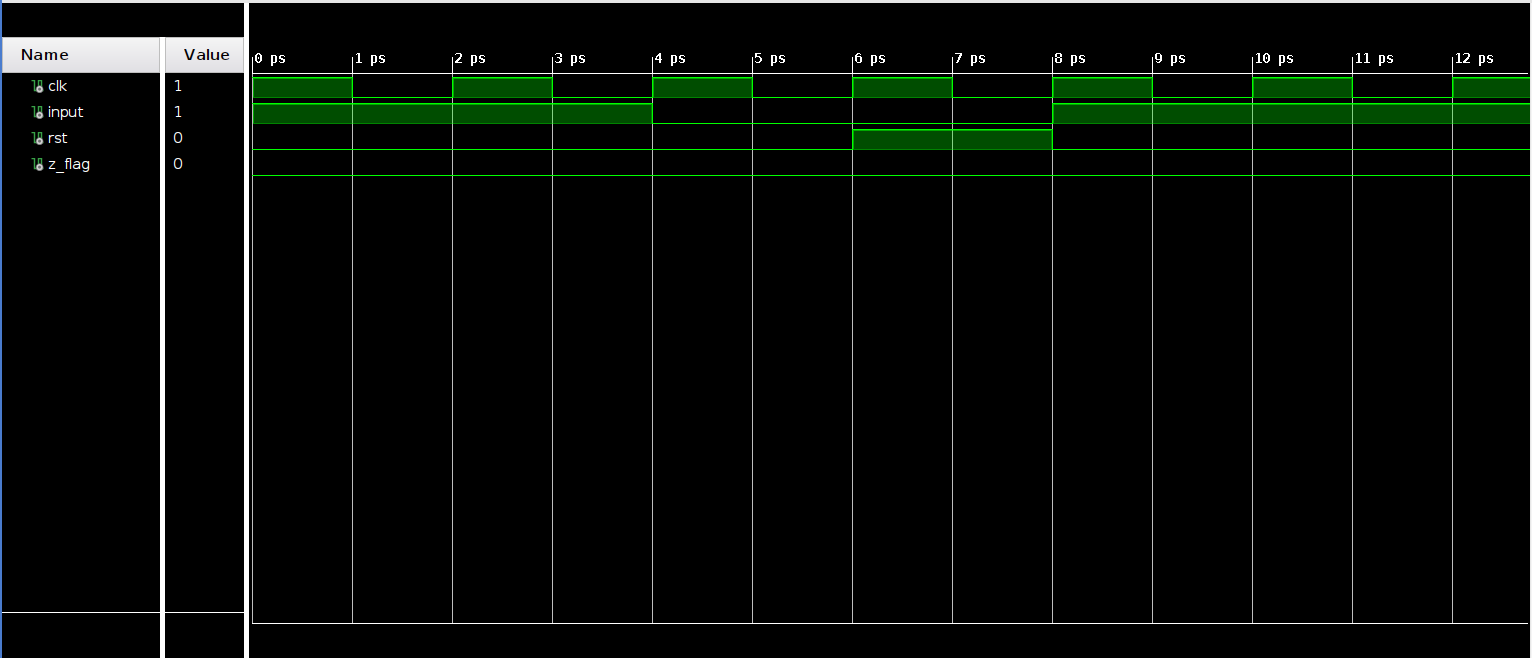
\includegraphics[scale=0.25]{images/no_overlap_reset.png}
    \caption{Simulation results of a base case receiving 11001 with no overlap, but receiving a reset}
    \label{fig:no_overlap_reset}
\end{figure}

\begin{figure}[H]
    \centering
    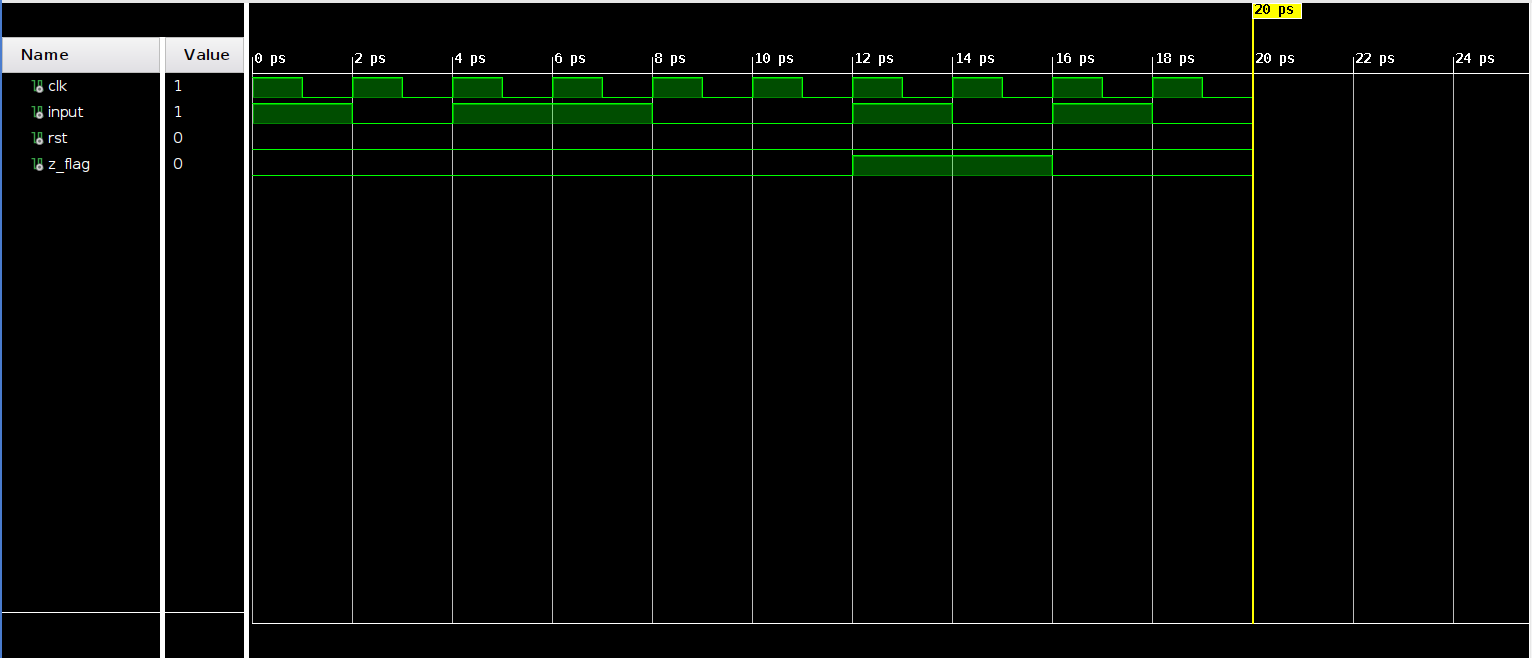
\includegraphics[scale=0.25]{images/10_sequence.png}
    \caption{Simulation results of receiving an input of 1011001010 to show detection in the middle of a sequence}
    \label{fig:10_sequence}
\end{figure}

\begin{figure}[H]
    \centering
    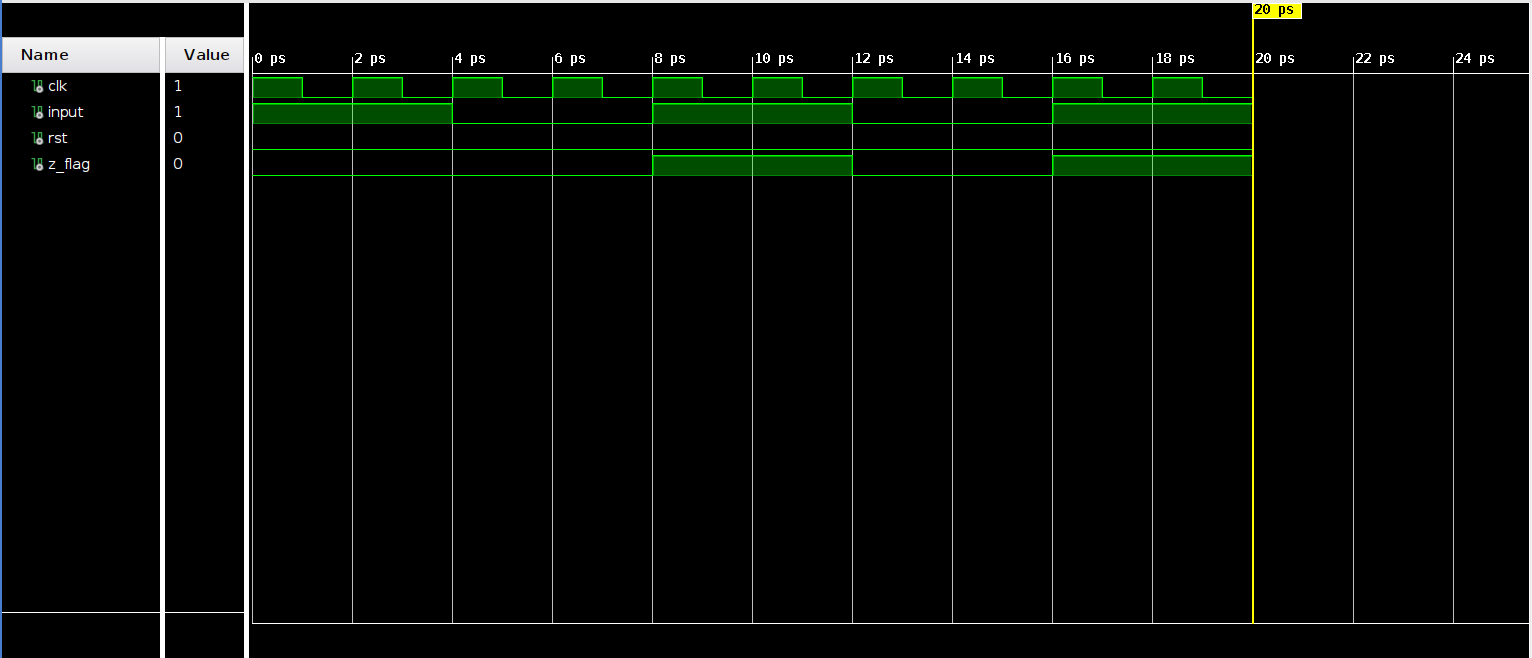
\includegraphics[scale=0.25]{images/overlap_no_reset.png}
    \caption{Simulation results of receiving 110011001 with overlap, but no reset}
    \label{fig:overlap_no_reset}
\end{figure}

\begin{figure}[H]
    \centering
    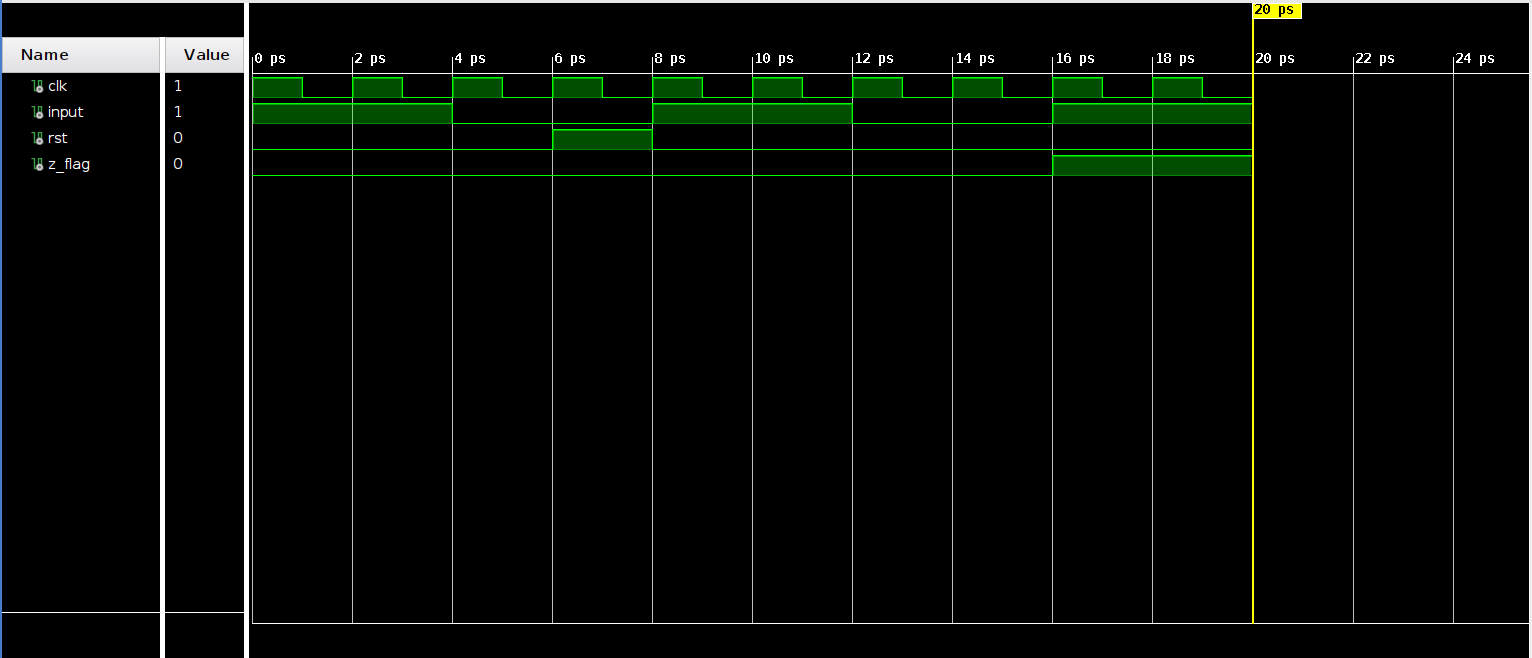
\includegraphics[scale=0.25]{images/overlap_reset.png}
    \caption{Simulation results of receiving 110011001 with overlap with a reset}
    \label{fig:overlap_reset}
\end{figure}

\section{Register Transfer Level Schematic}

Following the successful implementation of the design, it's important to analyse the generated RTL schematics. Figure \ref{fig:rtl_top_level} shows the top level design of the entire schematic.

\begin{figure}[H]
    \centering
    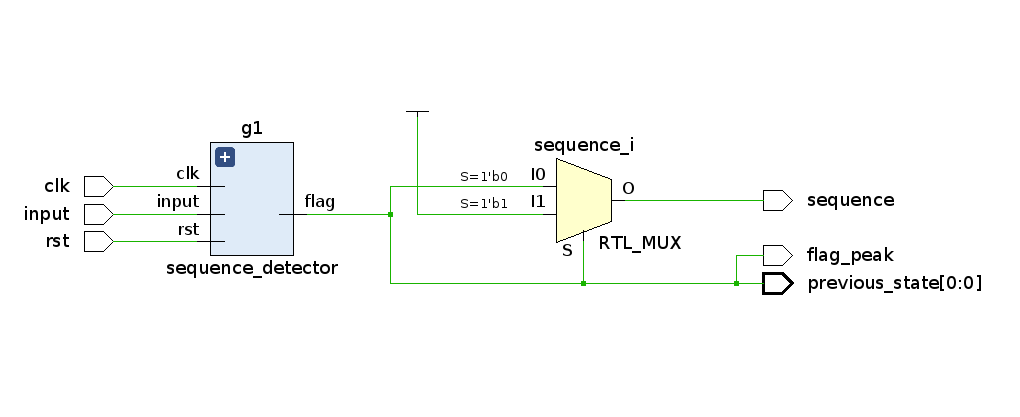
\includegraphics[scale=0.25]{images/rtl_top_level.png}
    \caption{RTL schematic of the top level design}
    \label{fig:rtl_top_level}
\end{figure}

As can be seen in figure \ref{fig:rtl_top_level}, the entire design can be broken into two main parts, each representing their respective FSM. The second FSM, receives an input from the first FSM, the input detector. It also receives an input clock line in order to main synchronicity, which becomes a serious issue for designing multi-FSM designs in Vivado. Within this figure, flag$\_$peak and previous$\_$state were signals used to peak at the states of both FSMs during testing. They can be ignored for simulation purposes. 

\begin{figure}[H]
    \centering
    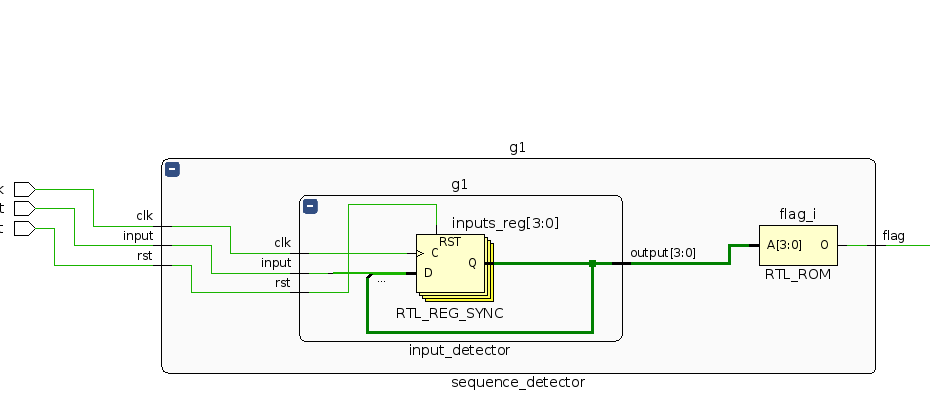
\includegraphics[scale=0.25]{images/rtl_fsm_1.png}
    \caption{Zoomed in RTL schematic for FSM 1}
    \label{fig:rtl_fsm_1}
\end{figure}

A zoomed in view of the RTL schematic for FSM 1 can be found in figure \ref{fig:rtl_fsm_1}. This comprises of a flip-flop feeding into a register which stores the input sequence, as described within the design architecture of this report.

\section{Synthesis Results}

\begin{figure}[H]
    \centering
    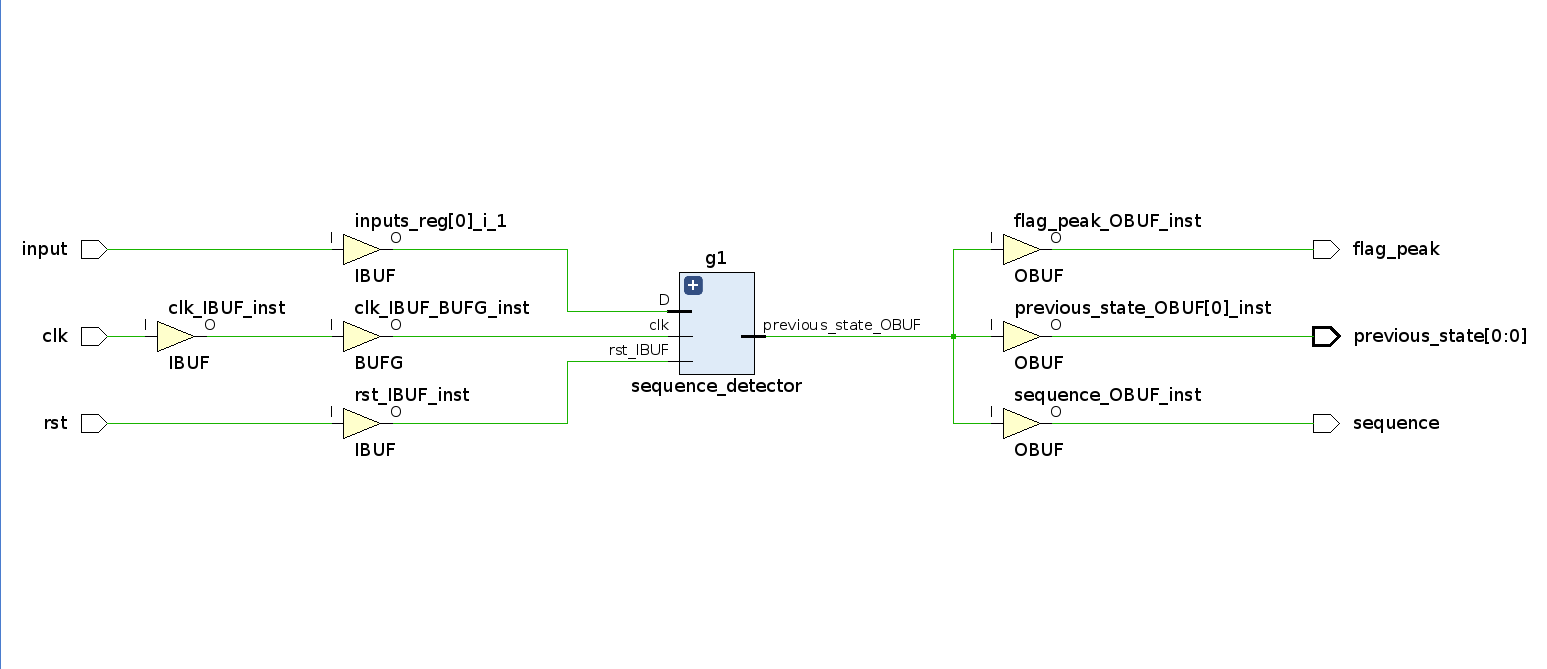
\includegraphics[scale=0.25]{images/synthesis_schematic.png}
    \caption{Synthesis schematic design}
    \label{fig:synthesis_schematic}
\end{figure}

Similar to the RTL schematics shown within their relevant section, figure \ref{fig:synthesis_schematic} shows the synthesized schematic. It also provides information as to the register configurations, and where the outputs and inputs are stored within the total design.

\begin{figure}[H]
    \centering
    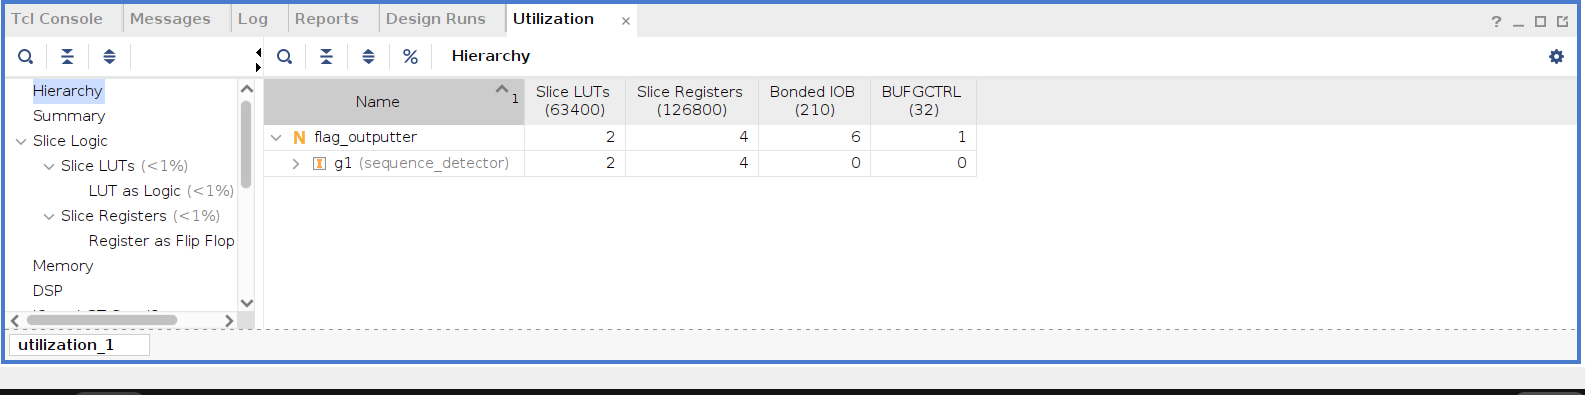
\includegraphics[scale=0.25]{images/synthesis_utilisation.png}
    \caption{Synthesis results displaying the memory utilisation}
    \label{fig:synthesis_utilisation}
\end{figure}

Figure \ref{fig:synthesis_utilisation} shows the total memory utilisation of this design. In perhaps the lowest memory consumption of this entire course, the prac 4 system requires 2 look-up tables used within FSM 1. Totalling in at 4 registers, less than 1$\%$ of the entire memory was utilised for full functionality.

\begin{figure}[H]
    \centering
    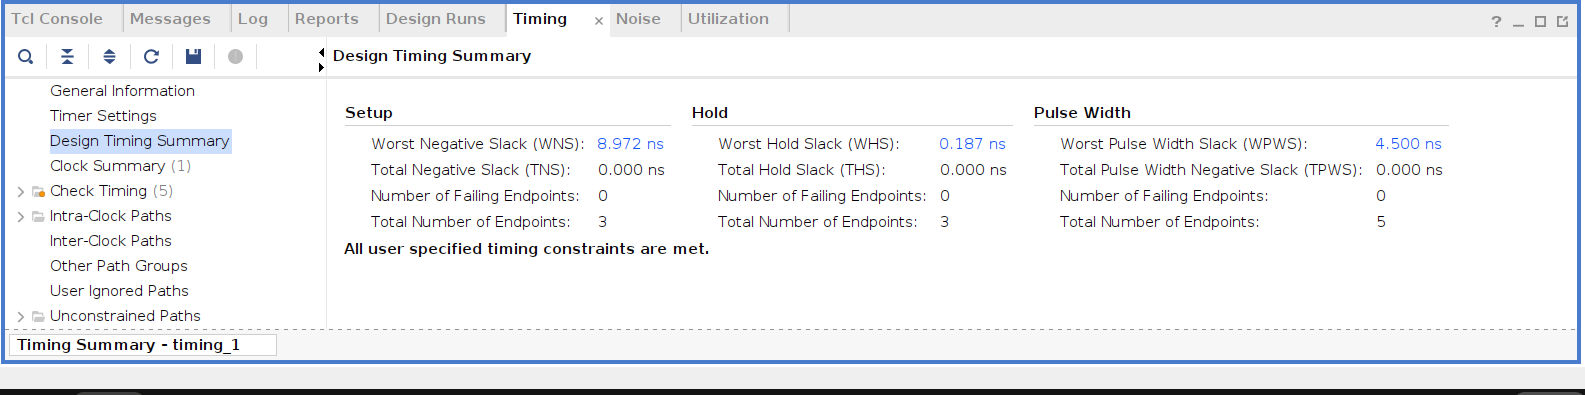
\includegraphics[scale=0.25]{images/clock_timing.png}
    \caption{Simulation results showing the timing slack. Note that there are no timing delays that exist within the design}
    \label{fig:clock_timing}
\end{figure}

Another important metric to evaluate is the timing slack that appears. In order to ascertain the synchronicity of the design, no timing slack can be present. Figure \ref{fig:clock_timing} shows that no slack is present within the design, indicating that no timing issues are present and synchronicity is maintained.

\section{Conclusion}

In conclusion, the system worked as expected. An FSM was generated that was able to output a high signal for two clock counts when the input into the FSM was "11001". This was achieved by using a double FSM system, where the first FSM detected the sequence and the second counted clock cycles. Everything worked as per the plan. 

See you next time for the final exciting epsiode of CSSE4011 prac reports!

\end{document}
